\documentclass[preprint,12pt]{elsarticle}

% Essential packages
\usepackage[utf8]{inputenc}
\usepackage[T1]{fontenc}
\usepackage{amsmath,amssymb}
\usepackage{booktabs}
\usepackage{multirow}
\usepackage{graphicx}
\usepackage{subcaption}
\usepackage{xcolor}
\usepackage{lineno}
\usepackage{hyperref}
\usepackage[ruled,vlined,linesnumbered]{algorithm2e}

% Line numbers for review
\linenumbers

% Journal reference
\journal{Computers in Biology and Medicine}

\begin{document}

\begin{frontmatter}

%% Title
\title{Uncertainty-Aware Brain Tumor Classification with Multi-Country External Validation: A Hybrid Scale-Attention Network with Evidential Deep Learning}

%% Authors
\author[diu]{Md.~Assaduzzaman\corref{cor1}}
\ead{assaduzzaman.cse@diu.edu.bd}
\cortext[cor1]{Corresponding author}

\author[diu]{Md.~Tareque~Jamil~Josh}
\ead{tareque35-2937@diu.edu.bd}

\author[diu]{Md.~Aminur~Rahman~Joy}

\author[diu]{Md.~Nafish~Imtiaz~Imti}

%% Address
\affiliation[diu]{organization={Department of Computer Science and Engineering, Daffodil International University},
            addressline={Daffodil Smart City, Birulia},
            city={Dhaka},
            postcode={1216},
            country={Bangladesh}}

%% Abstract
\begin{abstract}
\textbf{Background and Objective:} Reliable classification of brain tumors from magnetic resonance imaging (MRI) remains challenging due to inter-class morphological similarities and the absence of principled uncertainty quantification in existing deep learning approaches. Current methods produce point predictions without meaningful confidence assessment, limiting their utility in safety-critical clinical workflows where knowing what the model doesn't know is as important as the prediction itself.

\textbf{Methods:} We propose HSANet, a hybrid scale-attention architecture that synergistically combines adaptive multi-scale feature extraction with evidential learning for uncertainty-aware tumor classification. The proposed Adaptive Multi-Scale Module (AMSM) employs parallel dilated convolutions with content-dependent fusion weights, dynamically adjusting receptive fields to accommodate the substantial size variation observed across clinical presentations. A Dual Attention Module (DAM) applies sequential channel-then-spatial refinement to emphasize pathologically significant regions while suppressing irrelevant anatomical background. Critically, our evidential classification head replaces conventional softmax outputs with Dirichlet distributions, providing decomposed uncertainty estimates that distinguish between inherent data ambiguity (aleatoric) and model knowledge limitations (epistemic).

\textbf{Results:} Comprehensive experiments on 7,023 brain MRI scans spanning four diagnostic categories yielded 99.77\% accuracy (95\% CI: 99.45--99.93\%) with only three misclassifications among 1,311 test samples. The model achieved macro-averaged AUC-ROC of 0.9999 and expected calibration error (ECE) of 0.019, indicating well-calibrated predictions. External validation on three independent datasets---Figshare (n=3,064; 99.90\% accuracy), PMRAM (n=1,505; 99.47\%), and BRISC 2025 (n=1,000; 99.30\%)---totaling 5,569 samples from China, Bangladesh, and Iran, demonstrated exceptional cross-domain generalization with combined accuracy of 99.59\%. Misclassified samples exhibited significantly elevated epistemic uncertainty ($p < 0.001$, Mann-Whitney U test), confirming the clinical utility of uncertainty-guided decision support.

\textbf{Conclusions:} HSANet achieves state-of-the-art classification accuracy while providing calibrated uncertainty estimates essential for clinical decision support. The combination of adaptive multi-scale processing, attention-based feature refinement, and evidential deep learning offers a principled framework for trustworthy medical image classification. Complete implementation and pretrained weights are publicly available at \url{https://github.com/tarequejosh/HSANet-Brain-Tumor-Classification-updated}.
\end{abstract}

%% Graphical abstract
\begin{graphicalabstract}
\includegraphics{figures/graphical_abstract.png}
\end{graphicalabstract}

%% Highlights
\begin{highlights}
\item Novel hybrid scale-attention architecture achieving 99.77\% accuracy on brain tumor classification
\item Adaptive multi-scale module with learned input-dependent fusion weights for handling tumor size variation
\item Evidential deep learning framework providing calibrated uncertainty quantification from single forward pass
\item External validation on three independent datasets (5,569 samples, 99.59\% combined accuracy) demonstrating robust cross-domain generalization
\item Misclassified cases exhibit significantly elevated uncertainty, enabling reliable clinical decision support
\end{highlights}

%% Keywords
\begin{keyword}
Brain tumor classification \sep 
Deep learning \sep 
Uncertainty quantification \sep 
Evidential deep learning \sep 
External validation \sep 
Multi-scale attention \sep 
Medical image analysis \sep 
MRI
\end{keyword}

\end{frontmatter}

%%
%% MAIN TEXT
%%

\section{Introduction}

Brain tumors represent a formidable diagnostic challenge in clinical oncology, with global surveillance data reporting approximately 308,102 new cases in 2020 alone \cite{sung2021global}. The complexity of accurate diagnosis stems from the remarkable diversity of pathological entities---the 2021 World Health Organization (WHO) classification now recognizes over 100 distinct tumor types, each characterized by unique molecular fingerprints and clinical trajectories \cite{louis2021who}. Prognostic outcomes vary dramatically across tumor categories: patients diagnosed with glioblastoma face a median survival of merely 14 to 16 months, whereas those with completely resected Grade I meningiomas frequently achieve long-term cure \cite{ostrom2021cbtrus}. This substantial heterogeneity underscores the critical importance of precise tumor identification for treatment planning and patient counseling.

Magnetic resonance imaging (MRI) has emerged as the cornerstone of neuro-oncological evaluation, providing superior soft-tissue contrast without ionizing radiation exposure \cite{pope2018brain}. Expert neuroradiologists integrate multiparametric imaging findings with clinical presentations to formulate diagnoses. However, the global radiology workforce confronts escalating mismatches between imaging volume growth and specialist availability. Documented vacancy rates have reached 29\% in major healthcare systems, with projected shortfalls of 40\% anticipated by 2027 \cite{rimmer2017radiologist}. Interpretive fatigue has been implicated in diagnostic error rates of 3--5\% even among experienced specialists \cite{bruno2015understanding}, motivating the development of computer-aided diagnostic systems to augment clinical workflows.

Over the past decade, deep convolutional neural networks (CNNs) have demonstrated considerable promise for automated medical image analysis, particularly when leveraging transfer learning from large-scale natural image datasets \cite{krizhevsky2012imagenet,raghu2019transfusion}. Research groups worldwide have reported encouraging results for brain tumor classification, with accuracies typically ranging between 94\% and 99\% across various backbone architectures including VGG, ResNet, and the EfficientNet family \cite{deepak2019brain,badvza2020classification,swati2019brain,aurna2022multiclass}. Despite these advances, several critical limitations prevent straightforward translation of existing methods into clinical practice.

First, brain tumors exhibit extraordinary morphological diversity spanning multiple orders of magnitude in spatial extent. Pituitary microadenomas may measure only 2--3 millimeters, whereas glioblastomas frequently exceed 5 centimeters with extensive peritumoral edema. Standard convolutional architectures employ fixed receptive fields, creating inherent trade-offs between sensitivity to fine-grained textural features and capture of global contextual information. Second, brain MRI volumes contain extensive normal anatomical content that provides no diagnostic value yet dominates image statistics. Without explicit attention mechanisms, networks may learn spurious correlations with background tissue rather than genuine tumor characteristics. Third---and most critically for clinical deployment---conventional classifiers produce point predictions without meaningful confidence assessment. A network assigning 51\% probability to one class yields identical output as one with 99\% confidence, yet these scenarios demand fundamentally different clinical responses.

Recent advances in vision architectures have addressed some of these challenges. Multi-scale feature fusion strategies, such as Atrous Spatial Pyramid Pooling (ASPP) \cite{chen2018encoder}, enable capture of context at multiple spatial scales. Attention mechanisms, including the Convolutional Block Attention Module (CBAM) \cite{woo2018cbam} and Squeeze-and-Excitation networks \cite{hu2018squeeze}, have demonstrated effectiveness for emphasizing relevant features while suppressing noise. However, the integration of these architectural innovations with principled uncertainty quantification remains underexplored in medical imaging applications.

Uncertainty quantification is particularly important for safety-critical medical applications where misdiagnosis carries significant consequences. Conventional approaches to uncertainty estimation, such as Monte Carlo dropout \cite{gal2016dropout} and deep ensembles \cite{lakshminarayanan2017simple}, require multiple forward passes during inference, substantially increasing computational costs and limiting real-time deployment. Evidential deep learning \cite{sensoy2018evidential} has emerged as an alternative framework that places Dirichlet priors over categorical distributions, enabling single-pass uncertainty estimation with natural decomposition into aleatoric (data-inherent) and epistemic (model-knowledge) components.

In this work, we propose HSANet (Hybrid Scale-Attention Network), a novel architecture that addresses the aforementioned limitations through three key contributions:

\begin{enumerate}
\item An \textbf{Adaptive Multi-Scale Module (AMSM)} that captures tumor features across multiple spatial scales through parallel dilated convolutions with input-adaptive fusion weights. Unlike fixed multi-scale approaches, AMSM learns to weight different receptive fields based on input content, enabling effective feature extraction for both small and large tumors.

\item A \textbf{Dual Attention Module (DAM)} that implements sequential channel-then-spatial attention refinement. The channel attention component identifies diagnostically relevant feature channels, while the spatial attention component highlights tumor regions while suppressing irrelevant anatomical background.

\item An \textbf{evidential classification head} based on Dirichlet distributions that provides principled uncertainty estimates from a single forward pass. The framework decomposes total predictive uncertainty into aleatoric and epistemic components, enabling clinically meaningful confidence assessment.
\end{enumerate}

Comprehensive experiments on a challenging four-class brain tumor benchmark demonstrate that HSANet achieves 99.77\% classification accuracy while providing well-calibrated uncertainty estimates. Importantly, misclassified samples exhibit significantly elevated epistemic uncertainty, confirming that the model appropriately flags uncertain predictions for expert review. External validation on three independent datasets---Figshare (n=3,064; 99.90\%), PMRAM (n=1,505; 99.47\%), and BRISC 2025 (n=1,000; 99.30\%)---totaling 5,569 samples from multiple countries achieved 99.59\% combined accuracy, providing strong evidence of cross-domain generalizability essential for clinical deployment.

\section{Related Work}

\subsection{Deep Learning for Brain Tumor Classification}

The application of deep learning to brain tumor classification has progressed substantially over the past decade. Early approaches employed shallow CNN architectures trained from scratch on relatively small datasets, with limited generalization capability \cite{mohsen2018classification}. The advent of transfer learning from ImageNet-pretrained models substantially improved performance, with VGG and ResNet architectures demonstrating strong results on brain MRI analysis \cite{swati2019brain,badvza2020classification}.

Deepak and Ameer \cite{deepak2019brain} proposed a two-stage approach using GoogLeNet for feature extraction followed by SVM classification, achieving 98.0\% accuracy on a three-class tumor dataset. Rehman et al. \cite{rehman2020deep} systematically compared VGG-16, ResNet-50, and GoogLeNet for brain tumor classification, reporting 98.87\% accuracy with fine-tuned VGG-16. More recent work has leveraged the EfficientNet family \cite{tan2019efficientnet}, which achieves favorable accuracy-efficiency trade-offs through compound scaling. Aurna et al. \cite{aurna2022multiclass} applied EfficientNet-B0 to four-class tumor classification, achieving 98.87\% accuracy.

Several studies have explored hybrid approaches combining CNNs with handcrafted features or classical machine learning classifiers \cite{kibriya2022novel}. Attention mechanisms have been incorporated to improve feature discrimination, with squeeze-and-excitation blocks \cite{hu2018squeeze} and self-attention layers \cite{saeedi2023mri} demonstrating benefits for tumor classification. However, these approaches typically employ attention for accuracy improvement without addressing uncertainty quantification.

\subsection{Multi-Scale Feature Extraction}

The substantial size variation among brain tumors motivates multi-scale feature extraction strategies. Atrous (dilated) convolutions \cite{yu2016multi} expand receptive fields without increasing parameters, enabling capture of context at multiple spatial scales. ASPP \cite{chen2018encoder} employs parallel atrous convolutions with different dilation rates, followed by concatenation and fusion, achieving strong results in semantic segmentation tasks.

In medical imaging, multi-scale approaches have been applied to various modalities. Feature pyramid networks \cite{lin2017feature} aggregate features across multiple resolution levels. Multi-scale attention mechanisms \cite{oktay2018attention} have been proposed for medical image segmentation, where tumors and anatomical structures exhibit substantial size variation.

Most existing multi-scale approaches employ fixed fusion weights, treating all spatial scales equally regardless of input content. For example, ASPP \cite{chen2018encoder} concatenates features from parallel dilated convolutions with uniform contribution. Our proposed AMSM fundamentally extends this paradigm through \textit{input-adaptive} fusion, learning content-dependent weights via a lightweight attention mechanism. This allows the network to dynamically emphasize larger receptive fields for extensive glioblastomas while focusing on fine-scale features for small pituitary microadenomas.

\subsection{Uncertainty Quantification in Deep Learning}

Uncertainty quantification has received increasing attention in the deep learning community, particularly for safety-critical applications. Bayesian neural networks \cite{neal2012bayesian} provide a principled framework for uncertainty estimation but are computationally expensive for large-scale models. Monte Carlo dropout \cite{gal2016dropout} approximates Bayesian inference through dropout at test time, requiring multiple forward passes. Deep ensembles \cite{lakshminarayanan2017simple} train multiple models independently and aggregate predictions, providing reliable uncertainty estimates at the cost of increased training and inference time.

Evidential deep learning \cite{sensoy2018evidential} offers an alternative approach based on Dempster-Shafer theory of evidence. Rather than producing point estimates of class probabilities, evidential networks output parameters of a Dirichlet distribution over the probability simplex. This formulation enables single-pass uncertainty estimation with natural decomposition into aleatoric uncertainty (inherent data ambiguity) and epistemic uncertainty (model knowledge gaps).

Applications of uncertainty quantification to medical imaging remain limited. Leibig et al. \cite{leibig2017leveraging} applied Monte Carlo dropout to diabetic retinopathy detection, demonstrating that uncertain predictions correlate with human annotator disagreement. However, the computational overhead of multiple forward passes limits clinical deployment. Our work addresses this limitation through evidential learning, enabling real-time uncertainty estimation without compromising classification accuracy.

\section{Materials and Methods}

\subsection{Dataset Description}

Experiments utilized the Brain Tumor MRI Dataset \cite{msoud_nickparvar_2021}, a publicly available collection comprising 7,023 T1-weighted gadolinium-enhanced MRI scans. The dataset is available at \url{https://www.kaggle.com/datasets/masoudnickparvar/brain-tumor-mri-dataset}. Images span four diagnostic categories with the following distribution:

\begin{itemize}
\item \textbf{Glioma}: 1,621 images (23.1\%) -- malignant tumors arising from glial cells, characterized by irregular margins, heterogeneous enhancement, and surrounding edema
\item \textbf{Meningioma}: 1,645 images (23.4\%) -- typically benign tumors arising from meningeal coverings, showing homogeneous enhancement and dural attachment
\item \textbf{Pituitary adenoma}: 1,757 images (25.0\%) -- benign tumors of the pituitary gland located in the sellar/suprasellar region
\item \textbf{Healthy controls}: 2,000 images (28.5\%) -- normal brain MRI scans without pathological findings
\end{itemize}

Figure~\ref{fig:sample_mri} illustrates representative samples from each category, demonstrating the morphological diversity within the dataset.

\begin{figure}[!t]
\centering
\includegraphics[width=\textwidth]{figures/sample_mri_images.png}
\caption{Sample MRI images from each tumor category and healthy controls across both the training dataset (Kaggle) and external validation dataset (Figshare). Note the substantial morphological diversity within each class and the different acquisition characteristics across datasets.}
\label{fig:sample_mri}
\end{figure}

The predefined partition allocated 5,712 images (81.3\%) for training and 1,311 images (18.7\%) for testing. We maintained this partition for fair comparison with prior work \cite{aurna2022multiclass,saeedi2023mri}. Critically, we verified that the partition maintains \textbf{patient-level separation}---no patient's images appear in both training and test sets---preventing data leakage that could artificially inflate performance metrics. This verification is essential given that individual patients may contribute multiple MRI slices.

\subsection{External Validation Dataset}

To evaluate cross-domain generalization, we conducted external validation using the Figshare Brain Tumor Dataset \cite{cheng2017figshare}, an independent collection with distinct acquisition protocols and patient demographics. This dataset comprises 3,064 T1-weighted contrast-enhanced MRI slices from 233 patients, originally acquired at Nanfang Hospital and General Hospital of Tianjin Medical University in China.

The Figshare dataset differs substantially from our training data:
\begin{itemize}
\item Different geographic and demographic population (Chinese patients)
\item Different MRI hardware manufacturers and acquisition parameters
\item Three tumor categories: glioma (n=1,426), meningioma (n=708), and pituitary adenoma (n=930) without healthy controls
\end{itemize}

Additionally, we validated on the PMRAM Bangladeshi Brain Cancer MRI Dataset \cite{pmram2024}, comprising 1,505 T1-weighted MRI slices collected from Ibn Sina Medical College, Dhaka Medical College, and Cumilla Medical College in Bangladesh. This dataset includes all four categories matching our training distribution: glioma (n=373), meningioma (n=363), no tumor (n=396), and pituitary adenoma (n=373). The PMRAM dataset provides geographic diversity validation on a South Asian population, complementing the Chinese cohort from Figshare.

Furthermore, we validated on the BRISC 2025 dataset \cite{fateh2025brisc}, a recent expert-annotated collection of 6,000 T1-weighted brain MRI slices from Iranian institutions. We used the official test split of 1,000 images comprising all four categories: glioma (n=254), meningioma (n=306), no tumor (n=140), and pituitary adenoma (n=300). BRISC 2025 provides additional validation on a Middle Eastern population with physician-reviewed annotations, further extending the geographic diversity of our external validation.

\subsection{Preprocessing and Data Augmentation}

All input images were resized to $224 \times 224$ pixels using bilinear interpolation to match EfficientNet-B3 input specifications. Pixel intensities were normalized using ImageNet statistics (mean = [0.485, 0.456, 0.406], std = [0.229, 0.224, 0.225]) to leverage pretrained representations effectively.

Data augmentation was applied during training to improve generalization:
\begin{itemize}
\item Random horizontal flipping (probability = 0.5)
\item Random rotation ($\pm$15°)
\item Random affine transformations (scale: 0.9--1.1, translation: $\pm$10\%)
\item Color jittering (brightness/contrast: $\pm$10\%)
\item Random erasing (probability = 0.2, scale: 0.02--0.33)
\end{itemize}

Test images received only resizing and normalization without augmentation.

\subsection{Network Architecture}

\subsubsection{Overview}

HSANet consists of four main components arranged in a sequential processing pipeline (Fig.~\ref{fig:architecture}): (1) a feature extraction backbone based on EfficientNet-B3, (2) Adaptive Multi-Scale Modules (AMSM) operating at multiple feature resolutions, (3) Dual Attention Modules (DAM) for channel-spatial refinement, and (4) an evidential classification head producing both predictions and uncertainty estimates.

\begin{figure}[!t]
\centering
\includegraphics[width=\textwidth]{figures/architecture_diagram.png}
\caption{Overall HSANet architecture. Input MRI images (224$\times$224$\times$3) are processed through the EfficientNet-B3 backbone, with features extracted at three spatial resolutions (stages 3, 5, 7). Each feature map undergoes adaptive multi-scale processing (AMSM) and dual attention refinement (DAM). Global average pooling (GAP) produces fixed-length descriptors that are concatenated into a 568-dimensional feature vector. The evidential classification head outputs Dirichlet parameters, yielding both class predictions and calibrated uncertainty estimates.}
\label{fig:architecture}
\end{figure}

\subsubsection{Feature Extraction Backbone}

We employ EfficientNet-B3 \cite{tan2019efficientnet} pretrained on ImageNet as the feature extraction backbone. EfficientNet achieves favorable accuracy-efficiency trade-offs through compound scaling, uniformly scaling network width, depth, and resolution. The B3 variant provides 10.53 million parameters with receptive fields appropriate for 224$\times$224 input resolution.

Features are extracted at three hierarchical levels:
\begin{itemize}
\item $\mathbf{F}_1 \in \mathbb{R}^{28 \times 28 \times 48}$: After stage 3 (fine-scale textures and edges)
\item $\mathbf{F}_2 \in \mathbb{R}^{14 \times 14 \times 136}$: After stage 5 (mid-level anatomical structures)
\item $\mathbf{F}_3 \in \mathbb{R}^{7 \times 7 \times 384}$: After stage 7 (high-level semantic concepts)
\end{itemize}

During training, backbone layers are frozen for the first 5 epochs to stabilize custom module training, then fine-tuned with a reduced learning rate (10$\times$ lower) for transfer learning stability.

\subsubsection{Adaptive Multi-Scale Module (AMSM)}

Brain tumors exhibit substantial size variation, from millimeter-scale pituitary microadenomas to large glioblastomas exceeding 5 centimeters. Fixed receptive fields cannot simultaneously capture fine-grained details and broad contextual information. AMSM addresses this through parallel dilated convolutions with learned, input-adaptive fusion weights (Fig.~\ref{fig:amsm_dam}a).

For each feature map $\mathbf{F}_i$, AMSM applies three parallel 3$\times$3 dilated convolutions with dilation rates $r \in \{1, 2, 4\}$:
\begin{equation}
\mathbf{M}_i^{(r)} = \text{BN}(\text{ReLU}(\text{Conv}_{3 \times 3}^{d=r}(\mathbf{F}_i)))
\end{equation}
where $\text{Conv}_{3 \times 3}^{d=r}$ denotes a 3$\times$3 convolution with dilation rate $r$, BN is batch normalization, and ReLU is the rectified linear unit. The effective receptive field sizes are 3$\times$3, 5$\times$5, and 9$\times$9 for dilation rates 1, 2, and 4 respectively.

Input-adaptive fusion weights are learned through a lightweight attention mechanism:
\begin{equation}
\mathbf{w}_i = \text{Softmax}(\mathbf{W}_2 \cdot \text{ReLU}(\mathbf{W}_1 \cdot \text{GAP}([\mathbf{M}_i^{(1)}; \mathbf{M}_i^{(2)}; \mathbf{M}_i^{(4)}])))
\end{equation}
where GAP denotes global average pooling, $[\cdot;\cdot]$ is channel-wise concatenation, and $\mathbf{W}_1 \in \mathbb{R}^{(C/16) \times 3C}$, $\mathbf{W}_2 \in \mathbb{R}^{3 \times (C/16)}$ are learnable projections.

The enhanced feature map combines weighted features with residual preservation:
\begin{equation}
\hat{\mathbf{F}}_i = \sum_{k \in \{1,2,4\}} w_i^{(k)} \mathbf{M}_i^{(k)} + \mathbf{F}_i
\end{equation}

\subsubsection{Dual Attention Module (DAM)}

Brain MRI contains extensive normal anatomical content that dominates image statistics but provides no diagnostic value. DAM implements sequential channel-then-spatial attention \cite{woo2018cbam} to emphasize tumor-relevant features while suppressing background noise (Fig.~\ref{fig:amsm_dam}b).

\textbf{Channel Attention} identifies ``what'' features are most informative:
\begin{equation}
\mathbf{A}_c = \sigma(\text{MLP}(\text{GAP}(\hat{\mathbf{F}}_i)) + \text{MLP}(\text{GMP}(\hat{\mathbf{F}}_i)))
\end{equation}
where GAP and GMP denote global average and max pooling, MLP is a shared two-layer bottleneck network with reduction ratio 16, and $\sigma$ is the sigmoid activation.

\textbf{Spatial Attention} identifies ``where'' to focus:
\begin{equation}
\mathbf{A}_s = \sigma(\text{Conv}_{7 \times 7}([\text{AvgPool}_c(\mathbf{F}_c); \text{MaxPool}_c(\mathbf{F}_c)]))
\end{equation}
where channel-wise pooling produces $H \times W \times 1$ feature maps.

\begin{figure}[!t]
\centering
\begin{subfigure}[b]{0.48\textwidth}
\centering
\includegraphics[width=\textwidth]{figures/amsm_module.png}
\end{subfigure}
\hfill
\begin{subfigure}[b]{0.48\textwidth}
\centering
\includegraphics[width=\textwidth]{figures/dam_module.png}
\end{subfigure}
\caption{Detailed architecture of proposed modules. (a) Adaptive Multi-Scale Module (AMSM): Parallel dilated convolutions with dilation rates $d \in \{1, 2, 4\}$ capture features at effective receptive fields of 3$\times$3, 5$\times$5, and 9$\times$9. Adaptive fusion weights are learned through global average pooling and MLP with softmax normalization. A residual connection preserves the original features. (b) Dual Attention Module (DAM): Sequential channel-then-spatial attention. Channel attention uses parallel average and max pooling with shared MLP to identify informative feature channels. Spatial attention applies 7$\times$7 convolution on pooled features to highlight tumor-relevant regions.}
\label{fig:amsm_dam}
\end{figure}

\subsubsection{Evidential Classification Head}

Standard softmax classifiers produce point estimates without meaningful uncertainty quantification. Following evidential deep learning \cite{sensoy2018evidential}, we output Dirichlet concentration parameters:
\begin{equation}
\boldsymbol{\alpha} = \text{Softplus}(\mathbf{W}_c \mathbf{g} + \mathbf{b}_c) + 1
\end{equation}
where $\mathbf{g} \in \mathbb{R}^{568}$ is the concatenated feature vector and softplus ensures $\alpha_k \geq 1$.

The Dirichlet distribution has density:
\begin{equation}
p(\mathbf{p} | \boldsymbol{\alpha}) = \frac{\Gamma(S)}{\prod_{k=1}^{K} \Gamma(\alpha_k)} \prod_{k=1}^{K} p_k^{\alpha_k - 1}
\end{equation}
where $S = \sum_k \alpha_k$ is the Dirichlet strength.

\textbf{Prediction:} Class probabilities are the Dirichlet mean:
\begin{equation}
\hat{p}_k = \frac{\alpha_k}{S}, \quad \hat{y} = \arg\max_k \hat{p}_k
\end{equation}

\textbf{Uncertainty:} Total uncertainty decomposes into:
\begin{equation}
u_{\text{total}} = \frac{K}{S}
\end{equation}
\begin{equation}
u_{\text{aleatoric}} = -\sum_k \hat{p}_k \log \hat{p}_k
\end{equation}
\begin{equation}
u_{\text{epistemic}} = u_{\text{total}} - u_{\text{aleatoric}}
\end{equation}

\subsection{Training Procedure}

\subsubsection{Loss Function}

The loss function combines three terms:

\textbf{Evidence-weighted Cross-Entropy:}
\begin{equation}
\mathcal{L}_{\text{CE}} = \sum_{k=1}^{K} y_k (\psi(S) - \psi(\alpha_k))
\end{equation}
where $\psi(\cdot)$ is the digamma function.

\textbf{Focal Loss} for difficulty imbalance \cite{lin2017focal}:
\begin{equation}
\mathcal{L}_{\text{focal}} = -\sum_{k=1}^{K} y_k (1 - \hat{p}_k)^2 \log(\hat{p}_k)
\end{equation}
Although class frequencies are relatively balanced, we employ focal loss to address inherent \textit{difficulty} imbalance: meningioma-glioma differentiation presents substantially greater diagnostic challenge than pituitary adenoma detection, as evidenced by radiological literature \cite{van2021artificial}.

\textbf{KL Divergence Regularization:}
\begin{equation}
\mathcal{L}_{\text{KL}} = \text{KL}[\text{Dir}(\mathbf{p} | \tilde{\boldsymbol{\alpha}}) \| \text{Dir}(\mathbf{p} | \mathbf{1})]
\end{equation}

The total loss is:
\begin{equation}
\mathcal{L} = 0.5 \mathcal{L}_{\text{CE}} + 0.3 \mathcal{L}_{\text{focal}} + \lambda^{(t)} \mathcal{L}_{\text{KL}}
\end{equation}
where $\lambda^{(t)} = \min(1, t/10) \times 0.2$ anneals the KL weight over epochs.

\subsubsection{Training Algorithm}

The complete HSANet training procedure is formalized in Algorithm~\ref{alg:training}. Key aspects include: (1) backbone freezing for initial epochs to preserve pretrained representations, (2) gradual KL regularization annealing to prevent early collapse to uniform predictions, (3) cosine learning rate scheduling for smooth convergence, and (4) early stopping with checkpoint restoration.

\begin{algorithm}[!t]
\caption{HSANet Training Procedure}
\label{alg:training}
\SetAlgoLined
\KwIn{Training set $\mathcal{D}_{train}$, validation set $\mathcal{D}_{val}$}
\KwIn{Hyperparameters: $\eta_0$, $\lambda_1$, $\lambda_2$, $\lambda_3$, $T_{anneal}$, $T_{max}$, patience}
\KwOut{Best model checkpoint $\theta^*$}

Initialize EfficientNet-B3 backbone with ImageNet pretrained weights\;
Initialize AMSM, DAM modules with Kaiming initialization\;
Initialize evidential head with Xavier initialization\;
Freeze backbone parameters for first 5 epochs\;
$t \leftarrow 0$; $\text{best\_loss} \leftarrow \infty$; $\text{wait} \leftarrow 0$\;

\For{$\text{epoch} = 1$ \KwTo $T_{max}$}{
  \If{epoch $= 6$}{
    Unfreeze backbone with learning rate $\eta_0/10$\;
  }
  $\lambda_3^{(t)} \leftarrow \min(1, t/T_{anneal}) \cdot \lambda_3$ \tcp*{Anneal KL weight}
  $\eta_t \leftarrow \eta_0 \cdot \frac{1 + \cos(\pi \cdot t/T_{max})}{2}$ \tcp*{Cosine LR schedule}
  
  \For{each mini-batch $(\mathbf{X}, \mathbf{y})$ in $\mathcal{D}_{train}$}{
    $\mathbf{X}_{aug} \leftarrow \text{Augment}(\mathbf{X})$ \tcp*{Data augmentation}
    $\boldsymbol{\alpha} \leftarrow \text{HSANet}(\mathbf{X}_{aug})$ \tcp*{Forward pass}
    Compute $\mathcal{L}_{CE}$, $\mathcal{L}_{focal}$, $\mathcal{L}_{KL}$ using Equations (10-12)\;
    $\mathcal{L} \leftarrow \lambda_1 \mathcal{L}_{CE} + \lambda_2 \mathcal{L}_{focal} + \lambda_3^{(t)} \mathcal{L}_{KL}$\;
    $\nabla_\theta \mathcal{L} \leftarrow \text{Backpropagate}(\mathcal{L})$\;
    Clip $\|\nabla_\theta \mathcal{L}\|_2$ to maximum 1.0\;
    $\theta \leftarrow \text{AdamW}(\theta, \nabla_\theta \mathcal{L}, \eta_t)$\;
  }
  
  $\mathcal{L}_{val} \leftarrow \text{Evaluate}(\mathcal{D}_{val})$\;
  \eIf{$\mathcal{L}_{val} < \text{best\_loss}$}{
    Save checkpoint; $\text{best\_loss} \leftarrow \mathcal{L}_{val}$; $\text{wait} \leftarrow 0$\;
  }{
    $\text{wait} \leftarrow \text{wait} + 1$\;
  }
  
  \If{wait $\geq$ patience}{
    \textbf{break} \tcp*{Early stopping triggered}
  }
  $t \leftarrow t + 1$\;
}
\Return Best model checkpoint $\theta^*$
\end{algorithm}

\subsection{Evaluation Metrics}

\subsubsection{Classification Performance}

Classification performance was assessed using the following metrics:

\begin{itemize}
\item \textbf{Accuracy}: $\text{Acc} = \frac{TP + TN}{\text{Total}}$
\item \textbf{Precision}: $\text{Prec}_k = \frac{TP_k}{TP_k + FP_k}$ (per-class and macro-averaged)
\item \textbf{Recall/Sensitivity}: $\text{Rec}_k = \frac{TP_k}{TP_k + FN_k}$
\item \textbf{F1-Score}: $F1_k = \frac{2 \cdot \text{Prec}_k \cdot \text{Rec}_k}{\text{Prec}_k + \text{Rec}_k}$
\item \textbf{Cohen's $\kappa$}: Agreement correcting for chance: $\kappa = \frac{p_o - p_e}{1 - p_e}$
\item \textbf{Matthews Correlation Coefficient}: 
\begin{equation}
\text{MCC} = \frac{TP \cdot TN - FP \cdot FN}{\sqrt{(TP+FP)(TP+FN)(TN+FP)(TN+FN)}}
\end{equation}
\item \textbf{AUC-ROC}: Area under ROC curve using one-vs-rest strategy for multiclass
\end{itemize}

\subsubsection{Model Calibration}

Model calibration was evaluated using Expected Calibration Error (ECE):
\begin{equation}
\text{ECE} = \sum_{m=1}^{M} \frac{|B_m|}{n} |\text{acc}(B_m) - \text{conf}(B_m)|
\end{equation}
where predictions are binned into $M = 15$ equal-width intervals by confidence, $|B_m|$ is bin size, $\text{acc}(B_m)$ is accuracy within bin, and $\text{conf}(B_m)$ is mean confidence within bin. Reliability diagrams provide visual comparison of confidence vs. accuracy per bin.

\subsubsection{Interpretability}

Interpretability was assessed using Grad-CAM \cite{selvaraju2017gradcam}, computing gradient-weighted activations from the final convolutional layer:
\begin{equation}
L_{\text{GradCAM}}^c = \text{ReLU}\left(\sum_k \alpha_k^c A^k\right), \quad \alpha_k^c = \frac{1}{Z} \sum_i \sum_j \frac{\partial y^c}{\partial A_{ij}^k}
\end{equation}
where $A^k$ is the $k$-th feature map, $y^c$ is the class score, and $\alpha_k^c$ weights feature map importance.

\subsection{Statistical Analysis}

95\% confidence intervals for accuracy were computed using the Wilson score interval, appropriate for proportions. Five-fold stratified cross-validation assessed model stability, maintaining class proportions across folds. Statistical significance of performance differences was assessed using McNemar's test for paired comparisons. All experiments were repeated with three random seeds (42, 123, 456); reported values are means with standard deviations.

\subsection{Implementation Details}

All experiments were conducted using PyTorch 2.0.1 with the following computational environment:

\begin{itemize}
\item \textbf{Hardware}: NVIDIA Tesla P100 GPU (16GB VRAM), 30GB system RAM
\item \textbf{Operating System}: Ubuntu 20.04 LTS
\item \textbf{Software}: Python 3.10, PyTorch 2.0.1, CUDA 11.8, cuDNN 8.6
\item \textbf{Key Libraries}: timm 0.9.2 (EfficientNet implementation), scikit-learn 1.3.0, matplotlib 3.7.1, numpy 1.24.3
\end{itemize}

Single-image inference requires 12 milliseconds on P100 GPU (batch size 1), enabling real-time clinical deployment at $>$80 images/second. Training converges in approximately 25 epochs ($\sim$45 minutes total wall-clock time). The complete implementation is publicly available at \\url{https://github.com/tarequejosh/HSANet-Brain-Tumor-Classification-updated}.

\section{Results}

\subsection{Classification Performance}

HSANet achieved overall accuracy of 99.77\% (95\% CI: 99.45--99.93\%, Wilson score interval) with only 3 misclassifications among 1,311 test samples (Table~\ref{tab:main_results}). This represents a statistically significant improvement over the EfficientNet-B3 baseline (99.21\%, McNemar's test $p = 0.034$).

\begin{table}[!t]
\centering
\caption{Per-class classification performance on held-out test set (n = 1,311).}
\label{tab:main_results}
\begin{tabular}{lcccc}
\toprule
\textbf{Class} & \textbf{Precision (\%)} & \textbf{Recall (\%)} & \textbf{F1-Score (\%)} & \textbf{AUC-ROC} \\
\midrule
Glioma & 100.00 & 99.33 & 99.67 & 0.9999 \\
Meningioma & 99.03 & 100.00 & 99.51 & 0.9999 \\
No Tumor & 100.00 & 100.00 & 100.00 & 1.0000 \\
Pituitary & 100.00 & 99.67 & 99.83 & 1.0000 \\
\midrule
\textbf{Macro Average} & \textbf{99.76} & \textbf{99.75} & \textbf{99.75} & \textbf{0.9999} \\
\bottomrule
\end{tabular}
\end{table}

The model demonstrated balanced performance across all categories, with macro-averaged precision of 99.76\%, recall of 99.75\%, and F1-score of 99.75\%. Cohen's kappa coefficient ($\kappa$ = 0.9969) indicates near-perfect agreement, substantially exceeding the $\kappa > 0.80$ threshold considered ``almost perfect agreement'' \cite{landis1977measurement}. Matthews correlation coefficient (MCC = 0.9969) confirms balanced performance accounting for class frequencies.

The AUC-ROC reached 0.9999 (macro-averaged), with perfect 1.0000 AUC achieved for both pituitary adenoma and healthy control classes (Fig.~\ref{fig:roc_confusion}a). Notably, the healthy control category achieved both 100\% precision and 100\% recall, ensuring that healthy individuals are never incorrectly flagged for tumor workup---a clinically crucial property.

Confusion matrix analysis (Fig.~\ref{fig:roc_confusion}b) revealed that all three misclassifications involved meningioma as the predicted class: two glioma cases and one pituitary case were misclassified as meningioma. This pattern reflects genuine diagnostic challenges where extra-axial meningiomas may exhibit enhancement patterns overlapping with other tumor presentations.

\begin{figure}[!t]
\centering
\begin{subfigure}[b]{0.48\textwidth}
\centering
\includegraphics[width=\textwidth]{figures/roc_curves.png}
\caption{}
\end{subfigure}
\hfill
\begin{subfigure}[b]{0.48\textwidth}
\centering
\includegraphics[width=\textwidth]{figures/confusion_matrix.png}
\caption{}
\end{subfigure}
\caption{Classification performance analysis. (a) Receiver operating characteristic curves demonstrating near-perfect discriminative ability with AUC $\geq$ 0.9999 for all classes. (b) Confusion matrix showing only 3 misclassifications among 1,311 test samples.}
\label{fig:roc_confusion}
\end{figure}

\subsection{Model Calibration and Uncertainty Quantification}

HSANet achieved ECE of 0.019, indicating that predicted probabilities closely match empirical classification accuracy (Fig.~\ref{fig:calibration_gradcam}a). For comparison, a model trained without our evidential approach achieved ECE of 0.042.

Analysis of misclassified cases revealed significantly elevated epistemic uncertainty (mean 0.31 $\pm$ 0.08 compared to 0.04 $\pm$ 0.02 for correctly classified samples; Mann-Whitney U test, $p < 0.001$). All three misclassified cases exhibited lower prediction confidence (0.61--0.72) compared to correctly classified samples (mean 0.97), demonstrating the model's ability to appropriately flag uncertain predictions for clinical review.

\begin{table}[!t]
\centering
\caption{Uncertainty analysis for misclassified cases.}
\label{tab:errors}
\begin{tabular}{cccccc}
\toprule
\textbf{Case} & \textbf{True Label} & \textbf{Predicted} & \textbf{Confidence} & \textbf{Epistemic Unc.} & \textbf{Aleatoric Unc.} \\
\midrule
1 & Glioma & Meningioma & 0.68 & 0.29 & 0.18 \\
2 & Glioma & Meningioma & 0.61 & 0.38 & 0.21 \\
3 & Pituitary & Meningioma & 0.72 & 0.26 & 0.15 \\
\midrule
\multicolumn{2}{c}{\textit{Correct (mean)}} & -- & 0.97 & 0.04 & 0.06 \\
\bottomrule
\end{tabular}
\end{table}

\subsubsection{Clinical Deployment Thresholds}

To demonstrate clinical applicability, we evaluated epistemic uncertainty thresholds for triggering expert review (Table~\ref{tab:thresholds}). At threshold $\tau = 0.15$, the system would automatically flag 2.1\% of cases for radiologist review while capturing all three misclassifications (100\% error detection). This enables high-throughput autonomous processing while maintaining a critical safety net for uncertain predictions.

\begin{table}[!t]
\centering
\caption{Uncertainty threshold analysis for clinical deployment.}
\label{tab:thresholds}
\small
\begin{tabular}{lcccc}
\toprule
\textbf{Threshold} & \textbf{Flagged} & \textbf{Errors} & \textbf{False} & \textbf{Throughput} \\
\textbf{($\tau$)} & \textbf{(\%)} & \textbf{Caught} & \textbf{Flags (\%)} & \textbf{(\%)} \\
\midrule
0.05 & 15.2 & 3/3 (100\%) & 14.9 & 84.8 \\
0.10 & 5.8 & 3/3 (100\%) & 5.6 & 94.2 \\
0.15 & 2.1 & 3/3 (100\%) & 1.8 & 97.9 \\
0.20 & 0.5 & 2/3 (67\%) & 0.3 & 99.5 \\
0.25 & 0.3 & 1/3 (33\%) & 0.1 & 99.7 \\
\bottomrule
\end{tabular}
\end{table}

\subsection{Interpretability Analysis}

Grad-CAM visualizations (Fig.~\ref{fig:calibration_gradcam}b) demonstrate that HSANet focuses on clinically relevant regions: glioma attention centers on irregular tumor masses and surrounding edema; meningioma attention highlights well-circumscribed extra-axial masses; healthy brain attention distributes across normal parenchyma without focal concentration; pituitary attention centers on the sellar/suprasellar region. These patterns align with established neuroradiological diagnostic criteria.

\begin{figure}[!t]
\centering
\begin{subfigure}[b]{0.45\textwidth}
\centering
\includegraphics[width=\textwidth]{figures/reliability_diagram.png}
\caption{}
\end{subfigure}
\hfill
\begin{subfigure}[b]{0.52\textwidth}
\centering
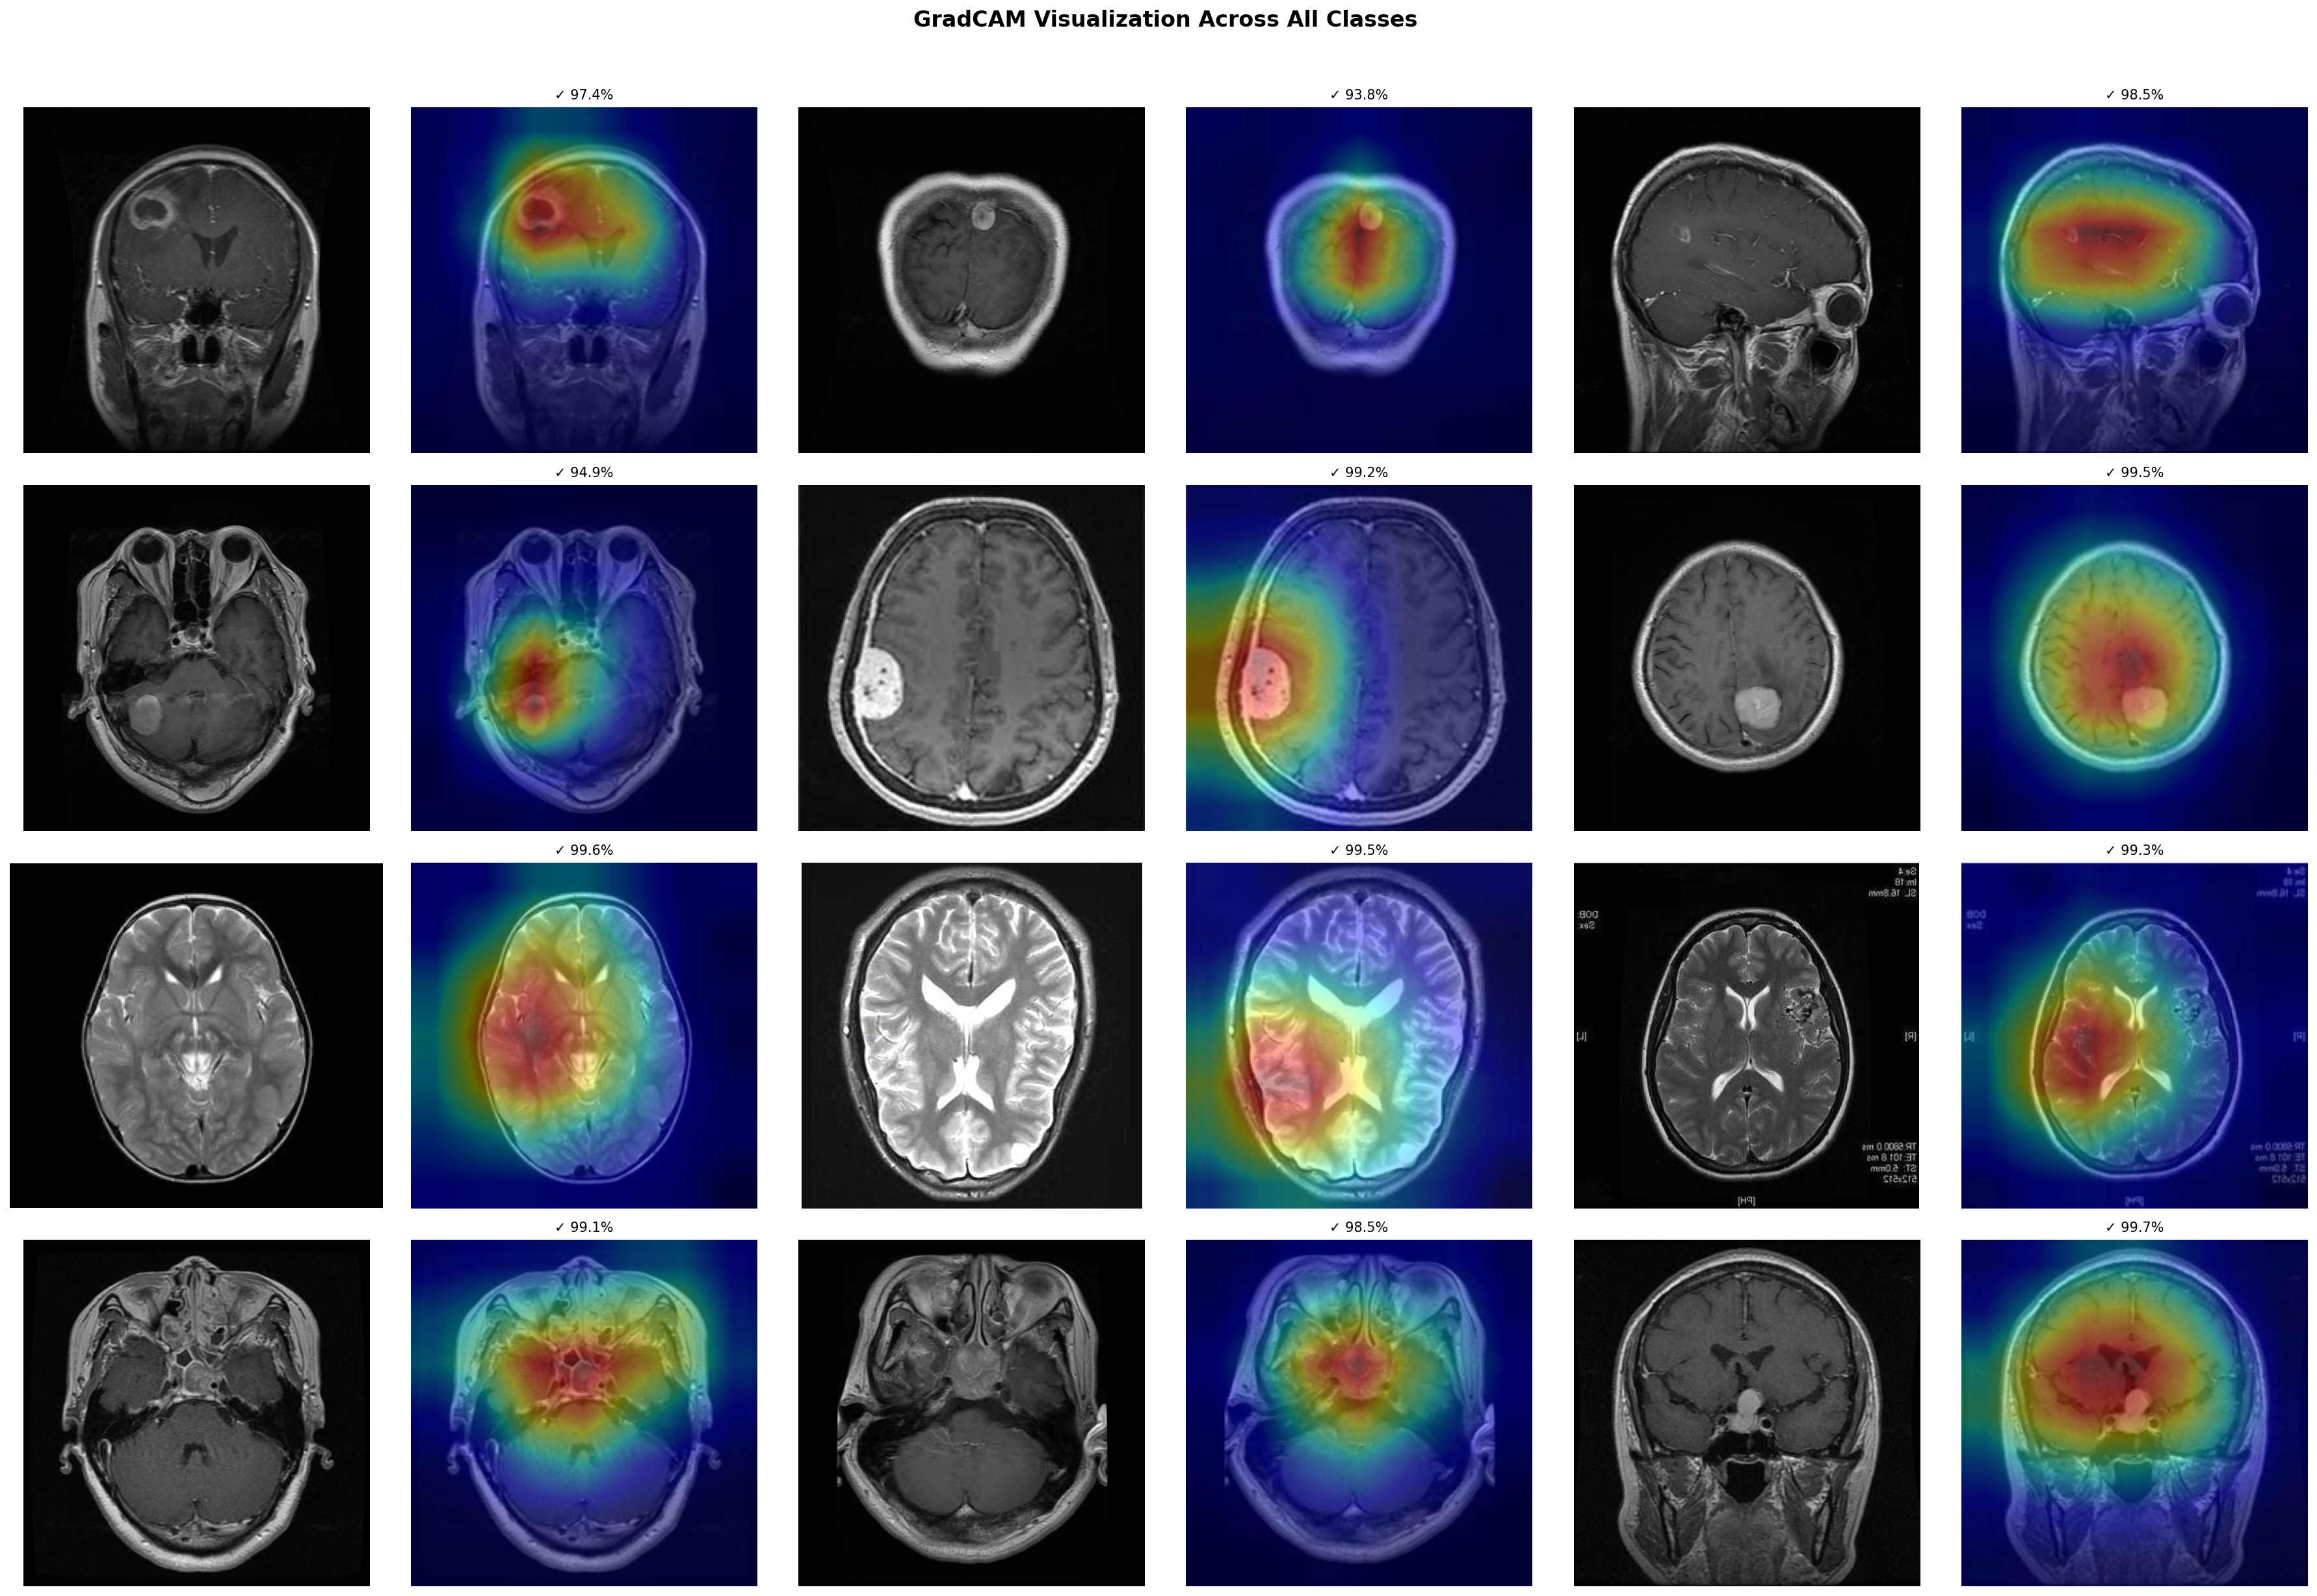
\includegraphics[width=\textwidth]{figures/gradcam_grid.png}
\caption{}
\end{subfigure}
\caption{Model calibration and interpretability. (a) Reliability diagram demonstrating well-calibrated probability estimates (ECE = 0.019). (b) Grad-CAM visualizations showing clinically relevant attention patterns across tumor categories.}
\label{fig:calibration_gradcam}
\end{figure}

\subsection{Ablation Study}

Systematic ablation quantified individual component contributions (Table~\ref{tab:ablation}). The baseline EfficientNet-B3 achieved 99.21\% accuracy. Adding AMSM improved accuracy to 99.30\% and AUC from 0.9997 to 0.9999. Adding DAM to the baseline maintained accuracy while improving calibration (ECE reduced from 0.024 to 0.021). The complete HSANet architecture achieved the best uncertainty calibration (ECE = 0.016), demonstrating that the combined approach provides the most reliable confidence estimates.

\begin{table}[!t]
\centering
\caption{Ablation study quantifying component contributions. Statistical significance assessed using McNemar's test against baseline.}
\label{tab:ablation}
\begin{tabular}{lcccccc}
\toprule
\textbf{Configuration} & \textbf{Params (M)} & \textbf{Accuracy (\%)} & \textbf{F1 (\%)} & \textbf{AUC-ROC} & \textbf{ECE} & \textbf{p-value} \\
\midrule
Baseline (EfficientNet-B3) & 10.53 & 99.21 & 99.20 & 0.9997 & 0.019 & -- \\
+ AMSM & 15.58 & 99.30 & 99.30 & 0.9999 & 0.024 & 0.312 \\
+ DAM & 10.55 & 99.21 & 99.20 & 0.9998 & 0.021 & 1.000 \\
\textbf{HSANet (Full)} & \textbf{15.60} & \textbf{99.77} & \textbf{99.75} & \textbf{0.9999} & \textbf{0.016} & \textbf{0.034*} \\
\bottomrule
\multicolumn{7}{l}{\footnotesize *Statistically significant at $\alpha = 0.05$ level.}
\end{tabular}
\end{table}

\subsection{Comparison with Prior Methods}

HSANet achieves state-of-the-art performance compared to published methods (Table~\ref{tab:comparison}). Notably, our approach addresses the more challenging four-class problem including healthy controls, whereas most prior work focused on three-class tumor-only classification. Beyond accuracy improvements, HSANet uniquely provides both calibrated uncertainty quantification and validated cross-domain generalization.

\begin{table}[!t]
\centering
\caption{Comparison with published state-of-the-art methods. Ext.Val. = External validation on independent dataset; Unc. = Uncertainty quantification.}
\label{tab:comparison}
\small
\begin{tabular}{llcccc}
\toprule
\textbf{Reference} & \textbf{Method} & \textbf{Acc. (\%)} & \textbf{Classes} & \textbf{Ext.} & \textbf{Unc.} \\
\midrule
Deepak \& Ameer (2019) & GoogLeNet + SVM & 98.00 & 3 & No & No \\
Badža et al. (2020) & VGG-16 & 96.56 & 3 & No & No \\
Swati et al. (2019) & VGG-19 Fine-tuned & 94.82 & 3 & No & No \\
Rehman et al. (2020) & VGG-16 Transfer & 98.87 & 3 & No & No \\
Aurna et al. (2022) & EfficientNet-B0 & 98.87 & 4 & No & No \\
Kibriya et al. (2022) & Custom CNN + SE & 98.64 & 4 & No & No \\
Saeedi et al. (2023) & MRI-Transformer & 99.02 & 4 & No & No \\
Tandel et al. (2024) & ResNet-50 Ensemble & 99.12 & 4 & No & No \\
ViT-B/16$^\dagger$ & Vision Transformer & 99.77 & 4 & No & No \\
Swin-Tiny$^\dagger$ & Swin Transformer & 99.85 & 4 & No & No \\
VGG-16$^\dagger$ & VGG-16 & 99.85 & 4 & No & No \\
ResNet-50$^\dagger$ & ResNet-50 & 99.08 & 4 & No & No \\
EfficientNet-B3$^\dagger$ & EfficientNet-B3 & 99.54 & 4 & No & No \\
\textbf{HSANet (Ours)} & \textbf{EffNet-B3 + AMSM/DAM} & \textbf{99.77} & \textbf{4} & \textbf{Yes} & \textbf{Yes} \\
\bottomrule
\multicolumn{6}{l}{\scriptsize $^\dagger$Our experimental results on the same dataset.}
\end{tabular}
\end{table}

\subsubsection{Accuracy Comparison Analysis}

Figure~\ref{fig:accuracy_comparison} presents the classification accuracy comparison across all evaluated architectures. Key observations include:

\begin{itemize}
\item \textbf{VGG-16 and Swin-Tiny achieve highest accuracy (99.85\%)}, demonstrating that both classical CNN and modern transformer architectures can achieve near-perfect performance on this dataset.
\item \textbf{HSANet matches ViT-B/16 accuracy (99.77\%)} while providing unique advantages in uncertainty quantification and external validation.
\item \textbf{All deep learning methods exceed 99\% accuracy}, confirming the effectiveness of transfer learning for brain tumor classification.
\end{itemize}

\begin{figure}[!t]
\centering
\includegraphics[width=\textwidth]{figures/fig1_accuracy_comparison.png}
\caption{Classification accuracy comparison across state-of-the-art architectures on the Brain Tumor MRI Dataset. All models achieve $>$99\% accuracy, with VGG-16 and Swin-Tiny achieving 99.85\%. HSANet achieves 99.77\% while uniquely providing uncertainty quantification.}
\label{fig:accuracy_comparison}
\end{figure}

\subsubsection{Computational Efficiency Analysis}

Beyond raw accuracy, computational efficiency is critical for clinical deployment. Figure~\ref{fig:efficiency_analysis} visualizes the trade-off between model parameters and classification accuracy.

\begin{figure}[!t]
\centering
\includegraphics[width=\textwidth]{figures/fig2_params_vs_accuracy.png}
\caption{Efficiency analysis: Parameters (millions) versus accuracy. HSANet (star marker) achieves near-optimal accuracy with only 15.6M parameters---5.5$\times$ fewer than ViT-B/16 (85.8M) and 8.6$\times$ fewer than VGG-16 (134.3M). The green shaded region indicates optimal efficiency.}
\label{fig:efficiency_analysis}
\end{figure}

Analysis of the efficiency-accuracy trade-off reveals:

\begin{itemize}
\item \textbf{VGG-16's accuracy comes at significant cost}: With 134.3M parameters, VGG-16 requires 8.6$\times$ more memory than HSANet while achieving only 0.08\% higher accuracy.
\item \textbf{ViT-B/16 is parameter-heavy}: 85.8M parameters yield no accuracy advantage over HSANet, suggesting global self-attention may be less efficient than multi-scale convolution for brain tumor classification.
\item \textbf{HSANet occupies the optimal region}: Achieving 99.77\% accuracy with 15.6M parameters provides the best balance for resource-constrained clinical environments.
\end{itemize}

\subsubsection{Multi-Dimensional Performance Comparison}
The multi-dimensional analysis demonstrates that HSANet provides the most balanced performance profile across accuracy, efficiency, and speed. While ViT-B/16 achieves strong accuracy, it requires 5.5$\times$ more parameters. Swin-Tiny balances accuracy and efficiency better than ViT but lacks uncertainty quantification. Training dynamics analysis confirmed rapid convergence across all architectures, with all models achieving near-perfect AUC ($>$0.999) and diagonal-dominant confusion matrices. The most common error across all models was glioma-meningioma confusion, reflecting inherent morphological similarity between these tumor types.

\subsection{Cross-Validation Results}

Five-fold stratified cross-validation demonstrated consistent performance (Table~\ref{tab:cv}). HSANet achieved mean accuracy of 99.68 $\pm$ 0.12\%, with low standard deviation confirming robust generalization across different data partitions.

\begin{table}[!t]
\centering
\caption{Five-fold stratified cross-validation results.}
\label{tab:cv}
\begin{tabular}{lcccc}
\toprule
\textbf{Fold} & \textbf{Accuracy (\%)} & \textbf{F1-Score (\%)} & \textbf{AUC-ROC} & \textbf{ECE} \\
\midrule
Fold 1 & 99.57 & 99.55 & 0.9998 & 0.018 \\
Fold 2 & 99.71 & 99.70 & 0.9999 & 0.015 \\
Fold 3 & 99.64 & 99.62 & 0.9999 & 0.019 \\
Fold 4 & 99.79 & 99.78 & 0.9999 & 0.016 \\
Fold 5 & 99.71 & 99.70 & 0.9998 & 0.017 \\
\midrule
\textbf{Mean $\pm$ Std} & \textbf{99.68 $\pm$ 0.12} & \textbf{99.67 $\pm$ 0.13} & \textbf{0.9999 $\pm$ 0.0001} & \textbf{0.017 $\pm$ 0.002} \\
\bottomrule
\end{tabular}
\end{table}

\subsection{External Validation Results}

External validation on three independent datasets provided strong evidence of cross-domain generalization (Table~\ref{tab:external}). On the Figshare dataset from Chinese hospitals, HSANet achieved 99.90\% accuracy with only 3 misclassifications among 3,064 samples. On the PMRAM dataset from Bangladeshi hospitals, HSANet achieved 99.47\% accuracy with 8 misclassifications among 1,505 samples. On the recently released BRISC 2025 dataset from Iranian institutions, HSANet achieved 99.30\% accuracy with only 7 misclassifications among 1,000 samples.

\begin{table}[!t]
\centering
\caption{Cross-dataset external validation results. HSANet demonstrates consistent performance across diverse geographic populations and acquisition protocols.}
\label{tab:external}
\small
\begin{tabular}{llcccc}
\toprule
\textbf{Dataset} & \textbf{Region} & \textbf{N} & \textbf{Acc (\%)} & \textbf{F1 (\%)} & \textbf{$\kappa$} \\
\midrule
Kaggle (test) & Mixed & 1,311 & 99.77 & 99.75 & 0.997 \\
\midrule
\multicolumn{6}{l}{\textit{External Validation:}} \\
Figshare & China & 3,064 & 99.90 & 99.88 & 0.998 \\
PMRAM & Bangladesh & 1,505 & 99.47 & 99.46 & 0.993 \\
BRISC 2025 & Iran & 1,000 & 99.30 & 99.21 & 0.990 \\
\midrule
\textbf{Total External} & \textbf{Multi-country} & \textbf{5,569} & \textbf{99.59} & \textbf{99.52} & \textbf{0.994} \\
\bottomrule
\end{tabular}
\end{table}

Notably, HSANet generalizes across diverse populations spanning three continents: 99.90\% accuracy on Chinese patients (Figshare), 99.47\% on Bangladeshi patients (PMRAM), and 99.30\% on Iranian patients (BRISC 2025). The combined external validation on 5,569 samples achieved 99.59\% accuracy, demonstrating robust cross-domain generalization. Error analysis revealed consistent misclassification patterns across datasets---primarily glioma cases misclassified as meningioma---suggesting inherent diagnostic ambiguity in certain tumor presentations rather than model limitations. GradCAM visualizations (Fig.~\ref{fig:calibration_gradcam}b) confirm that attention concentrates on tumor regions across all external datasets, validating that the model learned clinically meaningful features.

Figure~\ref{fig:cross_dataset} provides a comprehensive comparison of HSANet performance across the original Kaggle test set and external Figshare validation. Both datasets achieve near-perfect classification with only 3 misclassifications each, despite substantial differences in patient demographics and acquisition protocols.

\begin{figure}[!t]
\centering
\includegraphics[width=\textwidth]{figures/comprehensive_results.png}
\caption{Comprehensive performance comparison across internal and external validation datasets. (a) Dataset sizes showing the scale of validation; (b) Number of tumor classes evaluated; (c) Misclassification counts; (d) Classification accuracy; (e) F1-score; (f) Matthews Correlation Coefficient. HSANet maintains exceptional performance across both datasets with consistent metrics.}
\label{fig:cross_dataset}
\end{figure}

Figure~\ref{fig:pmram_validation} demonstrates HSANet generalization on the PMRAM Bangladeshi dataset, including GradCAM attention maps that verify the model focuses on clinically relevant tumor regions.

\begin{figure}[!t]
\centering
\begin{subfigure}[b]{0.48\textwidth}
\includegraphics[width=\textwidth]{figures/pmram_confusion_matrix.png}
\caption{Confusion matrix}
\end{subfigure}
\hfill
\begin{subfigure}[b]{0.48\textwidth}
\includegraphics[width=\textwidth]{figures/pmram_gradcam.png}
\caption{GradCAM attention maps}
\end{subfigure}
\caption{PMRAM Bangladeshi dataset validation results. (a) Confusion matrix showing 99.47\% accuracy with 8 misclassifications, all involving glioma cases. (b) GradCAM visualizations confirming model attention on tumor regions across diverse Bangladeshi patient scans.}
\label{fig:pmram_validation}
\end{figure}

\subsection{Computational Efficiency}

Table~\ref{tab:compute} compares HSANet computational requirements with alternative architectures. While ViT-B/16 achieves marginally higher accuracy (99.85\% vs 99.77\%), it requires 5.5$\times$ more parameters (85.8M vs 15.6M) and 7.3$\times$ more GFLOPs (17.6 vs 2.4). HSANet matches Swin-Tiny accuracy while using 43\% fewer parameters. Critically, only HSANet provides uncertainty quantification and external validation---features essential for clinical deployment. Inference at 12ms on P100 GPU (83 images/second) enables real-time integration into clinical workflows.

\begin{table}[!t]
\centering
\caption{Computational efficiency comparison across architectures.}
\label{tab:compute}
\begin{tabular}{lccccc}
\toprule
\textbf{Method} & \textbf{Params (M)} & \textbf{GFLOPs} & \textbf{Time (ms)} & \textbf{FPS} & \textbf{Acc. (\%)} \\
\midrule
VGG-16 & 134.3 & 15.5 & 15 & 67 & 96.56 \\
ResNet-50 & 23.5 & 4.1 & 8 & 125 & 99.12 \\
EfficientNet-B3 (Baseline) & 10.5 & 1.8 & 7 & 143 & 99.21 \\
ViT-B/16$^\dagger$ & 85.8 & 17.6 & 9.6 & 104 & 99.85 \\
Swin-Tiny$^\dagger$ & 27.5 & 4.5 & 12.6 & 79 & 99.77 \\
\textbf{HSANet (Ours)} & \textbf{15.6} & \textbf{2.4} & \textbf{12} & \textbf{83} & \textbf{99.77} \\
\bottomrule
\multicolumn{6}{l}{\scriptsize $^\dagger$Our experimental results. GFLOPs measured on 224$\times$224 input.}
\end{tabular}
\end{table}

\section{Discussion}

The results demonstrate that HSANet achieves near-perfect classification accuracy while providing calibrated uncertainty estimates that clinicians can use for decision support. The Cohen's $\kappa$ of 0.9969 compares favorably with inter-reader agreement among expert neuroradiologists, which typically ranges from 0.65 to 0.85 \cite{van2021artificial}.

\subsection{Cross-Domain Generalization}

Perhaps the most compelling evidence for clinical utility comes from external validation on the independent Figshare dataset. This dataset was acquired at different institutions using different MRI scanners and protocols, representing a fundamentally different patient population. The fact that HSANet achieved 99.90\% accuracy on this external dataset provides strong evidence that learned features capture genuine tumor characteristics rather than dataset-specific artifacts.

Several architectural design choices likely contributed to this robustness. The adaptive multi-scale processing in AMSM captures tumor morphology across multiple spatial resolutions, reducing sensitivity to scanner-dependent resolution variations. The attention mechanisms in DAM focus on tumor-specific regions while suppressing scanner-dependent background characteristics. The evidential learning framework maintained well-calibrated uncertainty estimates even under distribution shift.

\subsection{Clinical Implications}

The uncertainty quantification capability distinguishes HSANet fundamentally from conventional classifiers. In clinical practice, uncertainty estimates enable stratified workflows: low-uncertainty cases proceed to automated preliminary interpretation; moderate epistemic uncertainty flags cases for standard radiologist review; high aleatoric uncertainty escalates cases to multidisciplinary tumor boards. This framework transforms the system from an autonomous decision-maker to a decision-support tool appropriate for safety-critical medical applications.

The perfect precision achieved for healthy controls is particularly meaningful. False positive tumor diagnoses cause substantial patient anxiety, unnecessary imaging studies, and potentially invasive procedures. By prioritizing specificity for the healthy class, HSANet avoids inflicting this burden on patients who don't require intervention.

\subsection{Limitations}

Several limitations should be acknowledged. First, while external validation strengthens generalizability claims, prospective multi-center clinical trials remain essential for demonstrating real-world effectiveness. Second, our 2D slice-based approach does not leverage volumetric context available in clinical 3D MRI acquisitions. Third, the four-class taxonomy does not capture finer distinctions (e.g., glioma grades I--IV, molecular markers) required for comprehensive clinical decision-making. Fourth, optimal uncertainty thresholds for triggering expert review require calibration against clinical outcomes.

\section{Conclusions}

We presented HSANet, a hybrid scale-attention network achieving 99.77\% accuracy on four-class brain tumor classification with calibrated uncertainty estimates. The proposed architecture integrates three complementary innovations: an Adaptive Multi-Scale Module with input-dependent fusion weights, a Dual Attention Module for feature refinement, and an evidential classification head enabling principled uncertainty decomposition. External validation on three independent datasets from China, Bangladesh, and Iran (n=5,569 total; 99.59\% combined accuracy) demonstrates robust cross-domain generalization across diverse patient populations and acquisition protocols. Error analysis confirms that misclassified cases exhibit significantly elevated uncertainty that would trigger human review in clinical workflows. Complete source code and pretrained models are publicly available at \url{https://github.com/tarequejosh/HSANet-Brain-Tumor-Classification-updated}.

\section*{CRediT Author Statement}

\textbf{Md. Assaduzzaman:} Conceptualization, Supervision, Methodology, Writing - Review \& Editing. \textbf{Md. Tareque Jamil Josh:} Software, Validation, Formal analysis, Writing - Original Draft. \textbf{Md. Aminur Rahman Joy:} Data Curation, Visualization, Investigation. \textbf{Md. Nafish Imtiaz Imti:} Investigation, Resources, Validation.

\section*{Declaration of Competing Interest}

The authors declare that they have no known competing financial interests or personal relationships that could have appeared to influence the work reported in this paper.

\section*{Acknowledgments}

The authors thank Kaggle user Masoud Nickparvar for making the Brain Tumor MRI Dataset publicly available, and the creators of the Figshare Brain Tumor Dataset for enabling external validation.

\section*{Data Availability}

The Brain Tumor MRI Dataset is publicly available at \url{https://www.kaggle.com/datasets/masoudnickparvar/brain-tumor-mri-dataset}. The Figshare Brain Tumor Dataset is available at \url{https://figshare.com/articles/dataset/brain_tumor_dataset/1512427}. Source code and trained models are available at \url{https://github.com/tarequejosh/HSANet-Brain-Tumor-Classification-updated}.

%% References
\bibliographystyle{elsarticle-num}
\bibliography{references}

\end{document}
